% !TEX root = ../bachlor-arbeit.tex
The $S$-matrix calculus enables us to calculate the optical behavior of a stack if we know the optical behavior of all its layers in the form of their $S$-matrices. In section \ref{sec:s_mats} we derived the $S$-matrices of propagation through and interfaces between homogeneous isotropic materials. This calculation is based on the Fresnel equations and is therefore analytic. We cannot however calculate the $S$-matrix of a meta surface analytically. This results in a "Semi Analytic" Stacking Algorithm where the $S$-matrices of the meta surfaces need to be provided but the remaining $S$-matrices can be calculated based on the stack parameters.

\begin{figure}[H]
    \centering
    \includegraphics[width=.4\linewidth]{bg_two_layers}
    \caption{An example for a two meta layer stack. The top layer consist of rectangular gold particles arranged on a square matrix of period $\Lambda$. The bottom layer consist of rectangular holes in a gold sheet which are rotated by an angle of $\varphi$ in respect to the top layer. The two meta layers are separated by a glass spacer of thickness $d$.}
    \label{fig:bg:tow_layer}
\end{figure}

Importantly geometric transformations like rotation and mirroring can be applied directly to Jones matrices. For example let $\hat M$ be the Jones matrix of an optical component then the Jones matrix of the rotated component $\hat{M}_{\varphi}$ is calculated as:

\begin{equation}
    \hat{M}_{\varphi} = \hat \Theta(-\varphi) \, \hat{M} \, \hat \Theta(\varphi)
    \qq{where}
    \hat \Theta(\varphi) =
    \begin{pmatrix}
        \cos \varphi & \sin \varphi \\
        -\sin \varphi & \cos \varphi
    \end{pmatrix}
\end{equation}

On this basis we can rotate $S$-matrices in a similar manner:

\begin{equation}
    \hat S_\varphi =
    \begingroup
    \renewcommand*{\arraystretch}{1.5}
        \begin{pmatrix}
            \hat \Theta(-\varphi) \hat T^f \hat \Theta(\varphi)&
            \hat \Theta(-\varphi) \hat R^b \hat \Theta(\varphi)\\
            \hat \Theta(-\varphi) \hat R^f \hat \Theta(\varphi)&
            \hat \Theta(-\varphi) \hat T^b \hat \Theta(\varphi)
        \end{pmatrix}
    \endgroup
\end{equation}

Flipping and mirroring of $S$-matrices is done analogously. With all mathematical operations well defined we can write down SASA in pseudo code:
\\


\begin{figure}[H]
\begin{algorithm}[H]
    \SetAlgoLined
    \KwIn{Stack = $[\text{Layer}\, 0, \, \text{Layer 1}, \, \, \dots]$}
    \KwOut{Stack $S$-matrix}
    $S$-mats = $[\ ]$ \\
    \For{$i = 0$;  $i < \s{len}(\s{Stack})$;  $i = i+1$;}{
        \uIf{Stack$[i]$ \KwIs meta surface}{
            add layer $\hat S$ to $S$-mats
        } \Else {
            calculate propagation $S$-matrix $\hat S_{n_i,d_i}$ \\
            add $\hat S_{n_i,d_i}$ to $S$-mats
        }
        apply geometric transformations to added $S$-matrix \\
        calculate interface $S$-matrix $\hat S_{n_i,n_{i+1}}$ \\
        add $\hat S_{n_i,n_{i+1}}$ to $S$-mats
    }
    $\hat S = \mathbb 1$ \\
    \For{$i = 0$;  $i < \s{len}(\text{S-mats})$;  $i = i+1$;}{
        $\hat S = \hat S \star S$-mats$[i]$
    }
    \KwRet{$\hat S$}
\end{algorithm}
\caption*{SASA pseudocode: A Layer variable holds all the information of that layer, that is the $S$-matrix if its a meta layer and the refractive index $n$ and thickness $d$ otherwise.}
\end{figure}
\note{fix cursive?}


\newlparagraph{Conditions} \label{par:conditions}
For this algorithm to produce physical valid output some conditions need to be met. Equations that are boundary conditions to the algorithm will be marked bold. It has been shown \note{needs cite} that the $S$-matrix calculus can only be used when the meta materials in the stack interact with each other via the far field. That is only the zeroth diffraction order of a meta surface can be non evanescent and the higher orders need to have decayed enough when they reach the next meta surface.

\begin{boldequation} \label{bg:eq:lamda}
    \lambda > \max(n^f, n^b) \cdot \Lambda
\end{boldequation}

\eqref{bg:eq:lamda} ensures that only the zeroth diffraction order is non evanescent but additionally the spacer between the meta surfaces as seen in figure \ref{fig:bg:tow_layer} needs to be thick enough so that all non fundamental modes have decayed sufficiently. There is a calculation here \cite{Menzel2016} which concludes that if we require:

\begin{boldequation}
    e^{\Im(k_z)d} < e^{-2} \approx 0.14 \qq{then}
    d > \frac{\Lambda}{\pi \sqrt{1 - \frac{\Lambda^2 n^2}{\lambda^2}}}
\end{boldequation}

The factor $e^{-2}$ is chosen arbitrarily. A smaller value increases the agreement of the $S$-matrix calculus and more rigoros methods which also  take into account the near field.

\newlparagraph{Symmetries}
We can use the rotation matrix $\hat \Theta(\varphi)$ to examine the $S$-matrices of meta surfaces which satisfy certain symmetries. A meta surface of a $C^4$ symmetry for example square shape meta particles, is equivalent if rotated $90^\circ$ so the $S$-matrix should be the same too:

\begin{equation}
    \hat S \stackrel{!}{=} \hat S_{\pi/2} \qq{and}
    \hat \Theta(\pi/2) =
    \begin{pmatrix}
        \phantom{-} 0 & 1 \\
        -1 & 0
    \end{pmatrix}
\end{equation}
